\section{Resultados}

% ============== Experimentos ==========================
%------------------------------------------------
\begin{frame}
   \frametitle{Experimentos}
   \begin{block}{Detección del Danzante}
      \begin{itemize}
         \item Clasificadores
         \item Color
         \item Bordes
         \item Textura
      \end{itemize}
   \end{block}

\end{frame}

\begin{frame}
   \frametitle{Detección del Danzante: Clasificadores}
   
   \begin{table}[H]
   \centering
   \footnotesize {
   \begin{tabular}{*2c | *3c}
   \toprule
   \multicolumn{2}{c}{\textbf{Clasificador}} & \textbf{Adaboost} & \textbf{Random Forest} & \textbf{SVM} \tabularnewline 
    \midrule
   \textbf{Danza} & \textbf{\# de imágenes} & \textbf{\# de errores}  & \textbf{\# de errores} & \textbf{\# de errores} \tabularnewline 
   \midrule
    Qhapaq Chucho  & 640 & 52 & 77  & 63  \tabularnewline
    Qhapaq Qolla   & 640 & 36 & 53  & 56  \tabularnewline
    Contradanza    & 640 & 77 & 106 & 107 \tabularnewline
    Negrillo       & 640 & 27 & 44  & 105 \tabularnewline
   \midrule
   \textbf{TOTAL}       & \textbf{2560} & \textbf{192} & \textbf{280} & \textbf{331}\tabularnewline 
   \textbf{\% de error} &     --        & \textbf{7.50} & \textbf{10.94} & \textbf{12.93}\tabularnewline
   \bottomrule

   \end{tabular}
   }
   \end{table}
   Random Forest y SVM disminuyen la tasa de acierto en 3.44\% y 5.43\% respectivamente
\end{frame}

\begin{frame}
   \frametitle{Detección del Danzante: Color y Bordes}
   
   \begin{figure}[H]
   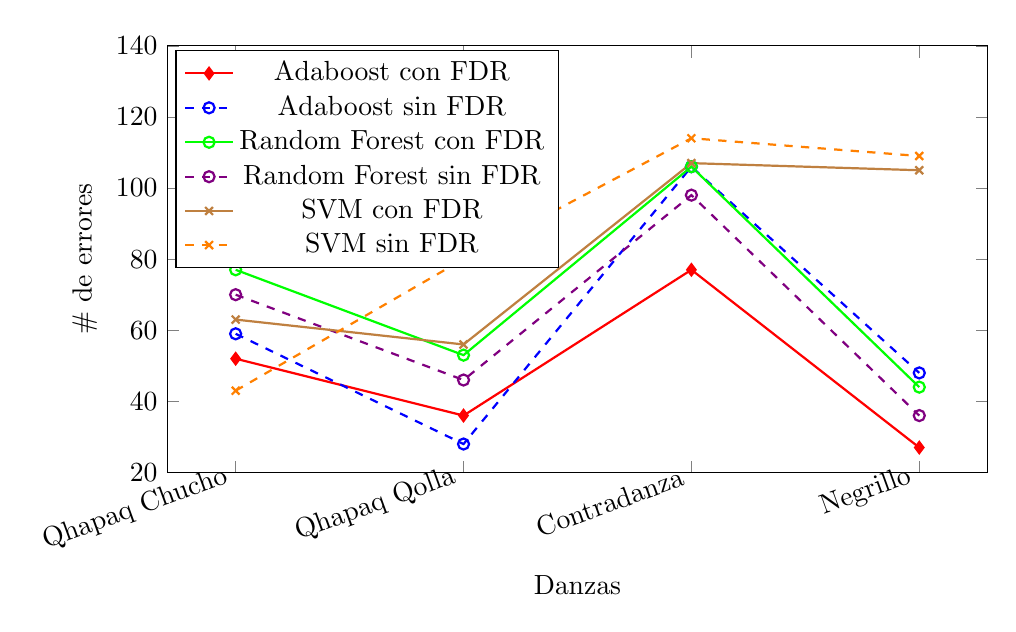
\begin{tikzpicture}
   \begin{axis}[legend style={at={(0.01,0.99)},anchor=north west},
               symbolic x coords={Qhapaq Chucho, Qhapaq Qolla, Contradanza, Negrillo}, xtick=data,
               x tick label style={rotate=20,anchor=east},
               ymin=20, ymax=140, width=12cm,
               height=7cm, xlabel = Danzas, ylabel = \# de errores
   ]

   \addplot[mark=diamond*,thick,red] coordinates {
      (Qhapaq Chucho, 52)
      (Qhapaq Qolla, 36)
      (Contradanza, 77)
      (Negrillo, 27)
   };
   \addlegendentry{Adaboost con FDR}
   \addplot[mark=o,mark options={solid},blue,thick,dashed] coordinates {
      (Qhapaq Chucho, 59)
      (Qhapaq Qolla, 28)
      (Contradanza, 106)
      (Negrillo, 48)
   };
   \addlegendentry{Adaboost sin FDR}

   \addplot[mark=o,thick,green] coordinates {
      (Qhapaq Chucho, 77)
      (Qhapaq Qolla, 53)
      (Contradanza, 106)
      (Negrillo, 44)
   };
   \addlegendentry{Random Forest con FDR}
   \addplot[mark=o,mark options={solid},violet,thick,dashed] coordinates {
      (Qhapaq Chucho, 70)
      (Qhapaq Qolla, 46)
      (Contradanza, 98)
      (Negrillo, 36)
   };
   \addlegendentry{Random Forest sin FDR}

   \addplot[mark=x,thick,brown] coordinates {
      (Qhapaq Chucho, 63)
      (Qhapaq Qolla, 56)
      (Contradanza, 107)
      (Negrillo, 105)
   };
   \addlegendentry{SVM con FDR}
   \addplot[mark=x,mark options={solid},orange,thick,dashed] coordinates {
      (Qhapaq Chucho, 43)
      (Qhapaq Qolla, 80)
      (Contradanza, 114)
      (Negrillo, 109)
   };
   \addlegendentry{SVM sin FDR}

   \end{axis}
   \end{tikzpicture}
\end{figure}

\end{frame}

% ============== DEMO ==========================

\begin{frame}

\begin{beamercolorbox}[sep=8pt,center,colsep=-4bp,rounded=true,shadow=true]{title}
        \usebeamerfont{title} Demo  \par%
        \ifx\insertsubtitle\@empty%
        \else%
        \vskip0.25em%
        {\usebeamerfont{subtitle}\usebeamercolor[fg]{subtitle}\insertsubtitle\par}%
      \fi%     
     \end{beamercolorbox}%

\end{frame}

% ============== Detalles Técnicos ==========================
%------------------------------------------------
\begin{frame}
\frametitle{Detalles Técnicos}
\FontDetalleTecnico
\begin{block}{Hardware}

   \begin{itemize}
   \item \textbf{Cámara:} Nikon D7200.
   \item \textbf{Notebook:} Toshiba Satellite S845. Procesador Intel Core-i5 3rd generation/2.5 GHz, 4Gb RAM DDR3.
   \item \textbf{Notebook:} Lenovo Y700. Procesador Intel Core-i7 6rd generation/3.5 GHz, 8Gb RAM DDR4.
   \end{itemize}
   
\end{block}

\begin{block}{Software}
   \begin{itemize}
   \item \textbf{Sistema Operativo:} Ubuntu 16.04.1 LTS x86\_64
   \item \textbf{Lenguaje de Programación:} Python 2.7
   \item \textbf{Librerías:} Opencv 3.0.0, NumPy 1.11.2, SciPy 0.17.0, SciKitLearn 0.18 y SciKitImage 0.12.3
   \item \textbf{Controlador de versiones:} Git 2.10
   \end{itemize}
   
\end{block}

\end{frame}
%------------------------------------------------


